%=================================================================================================
%=							              AGRADECIMENTOS						     			 =
%=================================================================================================


\begin{agradecimentos}

Este trabalho foi possível em decorrência de muitas vivências que obtive durante a minha vida.

Agradeço ao meu Orientador Victor Dmitriev e Coorientador Ronaldo Zampolo pela orientação neste trabalho.

Agradeço aos amigos do Laboratório de Nanofotônica e Nanoeletrônica pelo suporte no desenvolvimento da pesquisa que resultou no presente trabalho e do contato com o Programa de Pós-Graduação em \imprimircurso. Em especial: Gianni Portela, Geraldo Melo e Wagner Castro.

Agradeço a todos os meus professores que me proporcionaram um grande aprendizado ao decorrer da graduação. Em especial: Roberto Menezes, Washington Sousa, Claudomiro Barbosa e Thiago Mota.

Agradeço a minha família: Deuza (minha mãe), José João (meu pai), Natália e Jéssica (minhas irmãs).

Agradeço aos meus amigos que me acompanharam na graduação, em especial: Rodrigo Dutra, Edilberto Oliveira, Marcio Muniz, Abel Massunanga.

Agradeço aos meus amigos do projeto de divulgação científica Clube de Astronomia do Pará (CAP), pelos esforços e companheirismo na divulgação científica e combate às \textit{pseudociências}.

Agradeço, também, a mim mesmo pelo esforço e intensa curiosidade em procurar saber \textit{como as coisas funcionam}, característica que se manifestou em mim desde que me entendo por gente, o que me permitiu a sempre investigar novos desafios.

Esse trabalho teve o suporte do Conselho Nacional de Desenvolvimento Científico e Tecnológico (CNPq), da Pró-Reitoria de Pesquisa (PROPESP) e da Universidade Federal do Pará (UFPA).

\vfill

\begin{figure}[H]
    \centering
    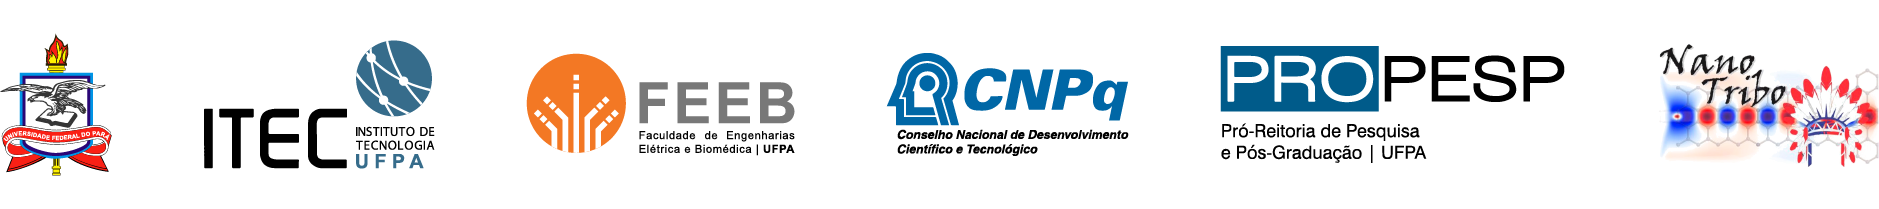
\includegraphics{04-Figuras/Agradecimentos.png}
\end{figure}

\vfill


\end{agradecimentos}